\section{性能評価}
コンテストから提供されるテスト画像649枚に対してUltra96-V2ボード上で推論を実行した.
実行時間の評価における設定項目は以下の通りである.
\begin{itemize}
    \item{DPU:B2304@200/400MHz}
    \item{推論画像サイズ:320*640}
    \item{BATCH\_SIZE:130}
\end{itemize}
\subsection{実行時間}
シングルスレッド実装において,前処理,推論処理,後処理はそれぞれ11.857ms,54.823ms,18.445msであった.
マルチスレッド実装における前処理〜推論処理〜後処理の平均時間は57.928msであった.
マルチスレッド実装によって1枚あたりの平均処理時間が大幅に短縮されていることが確認できた.

\subsection{実行結果}
図\ref{estimate_result}に入力画像と推論結果,および推論結果を入力画像に合成したものの1例を示す.
\begin{figure}[b]
    \label{estimate_result}
    \caption{推論結果}
    \begin{minipage}{0.33\hsize}
     \begin{center}
      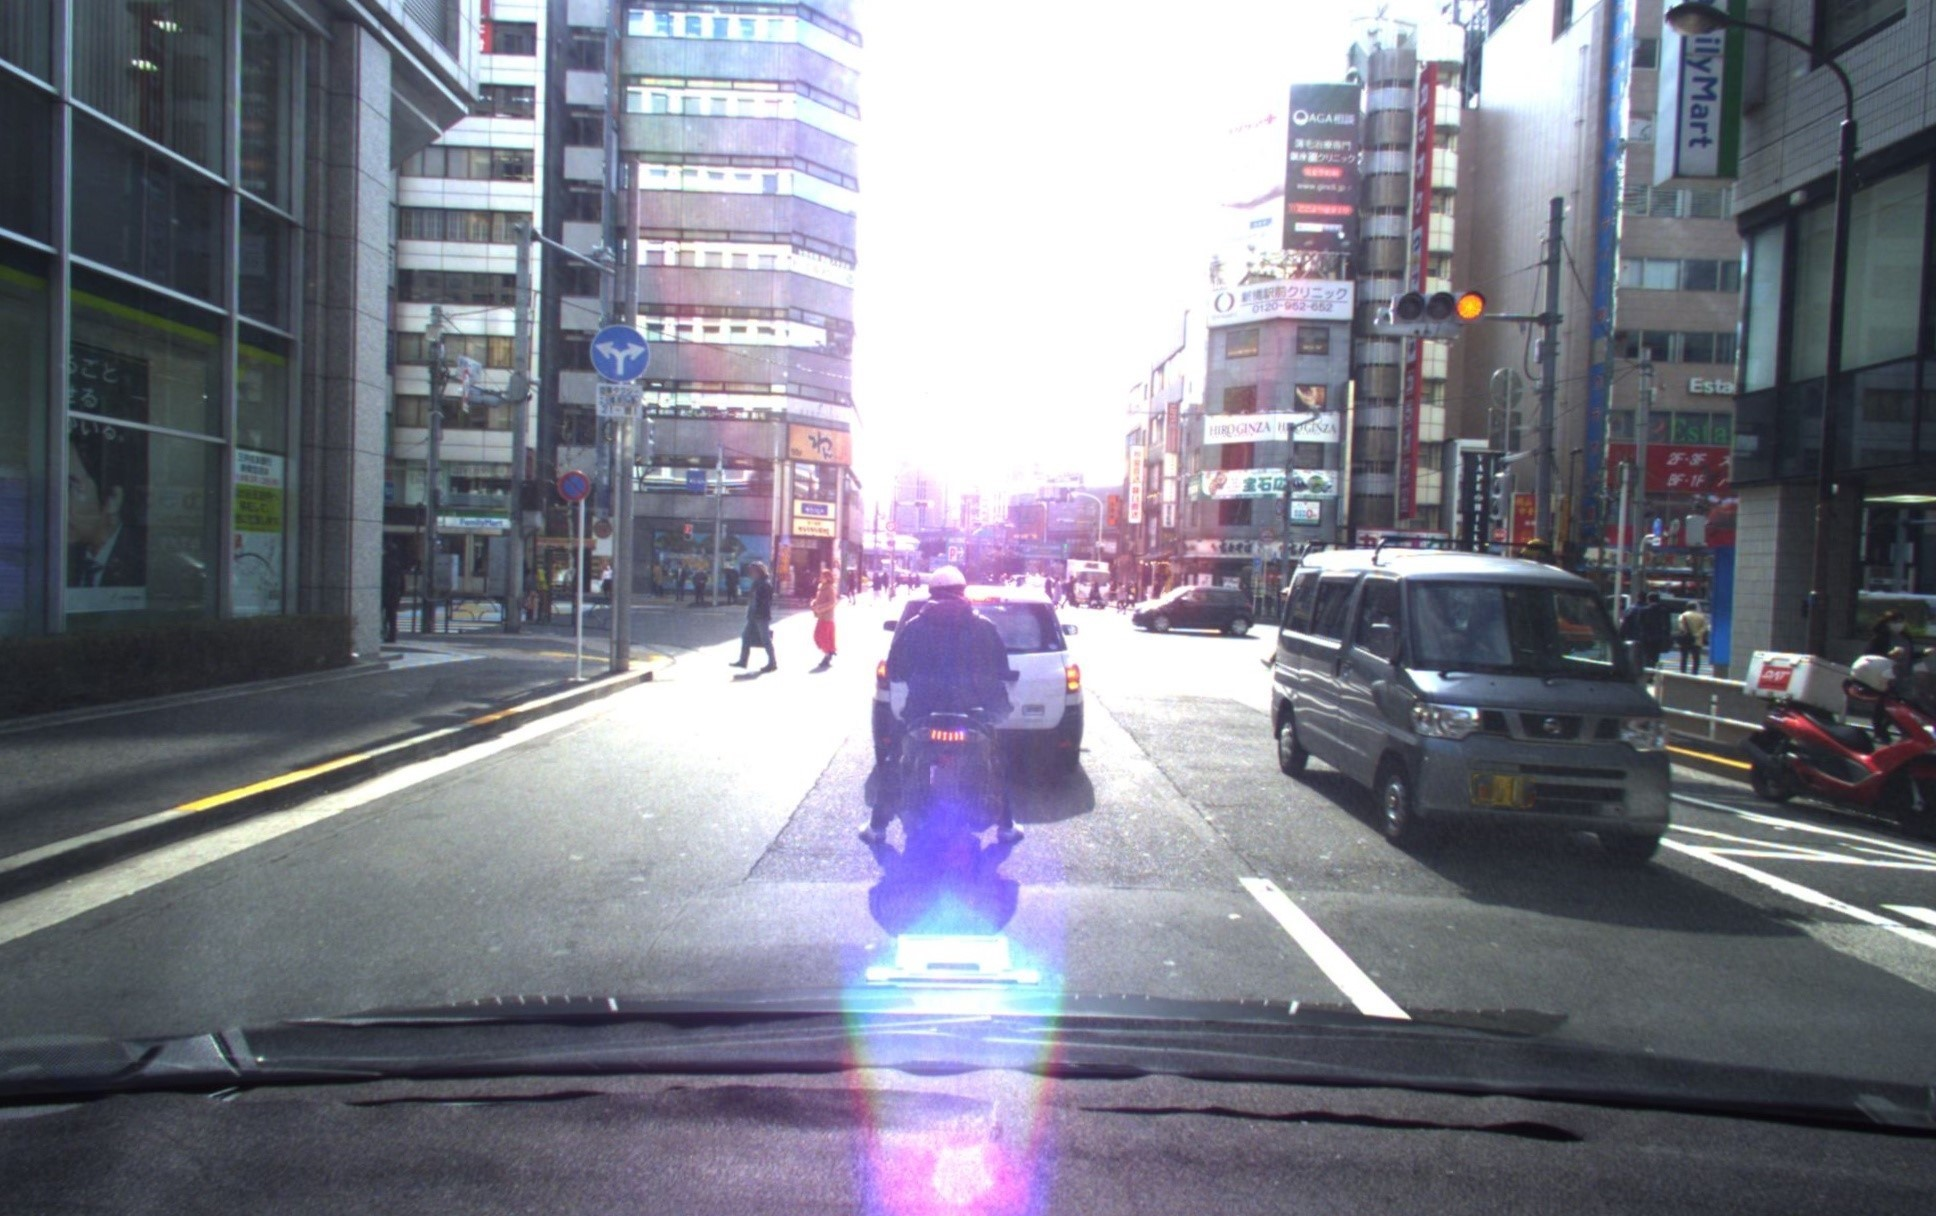
\includegraphics[width=60mm]{./figures/orig.jpg}
     \end{center}
    \end{minipage}
    \begin{minipage}{0.33\hsize}
     \begin{center}
      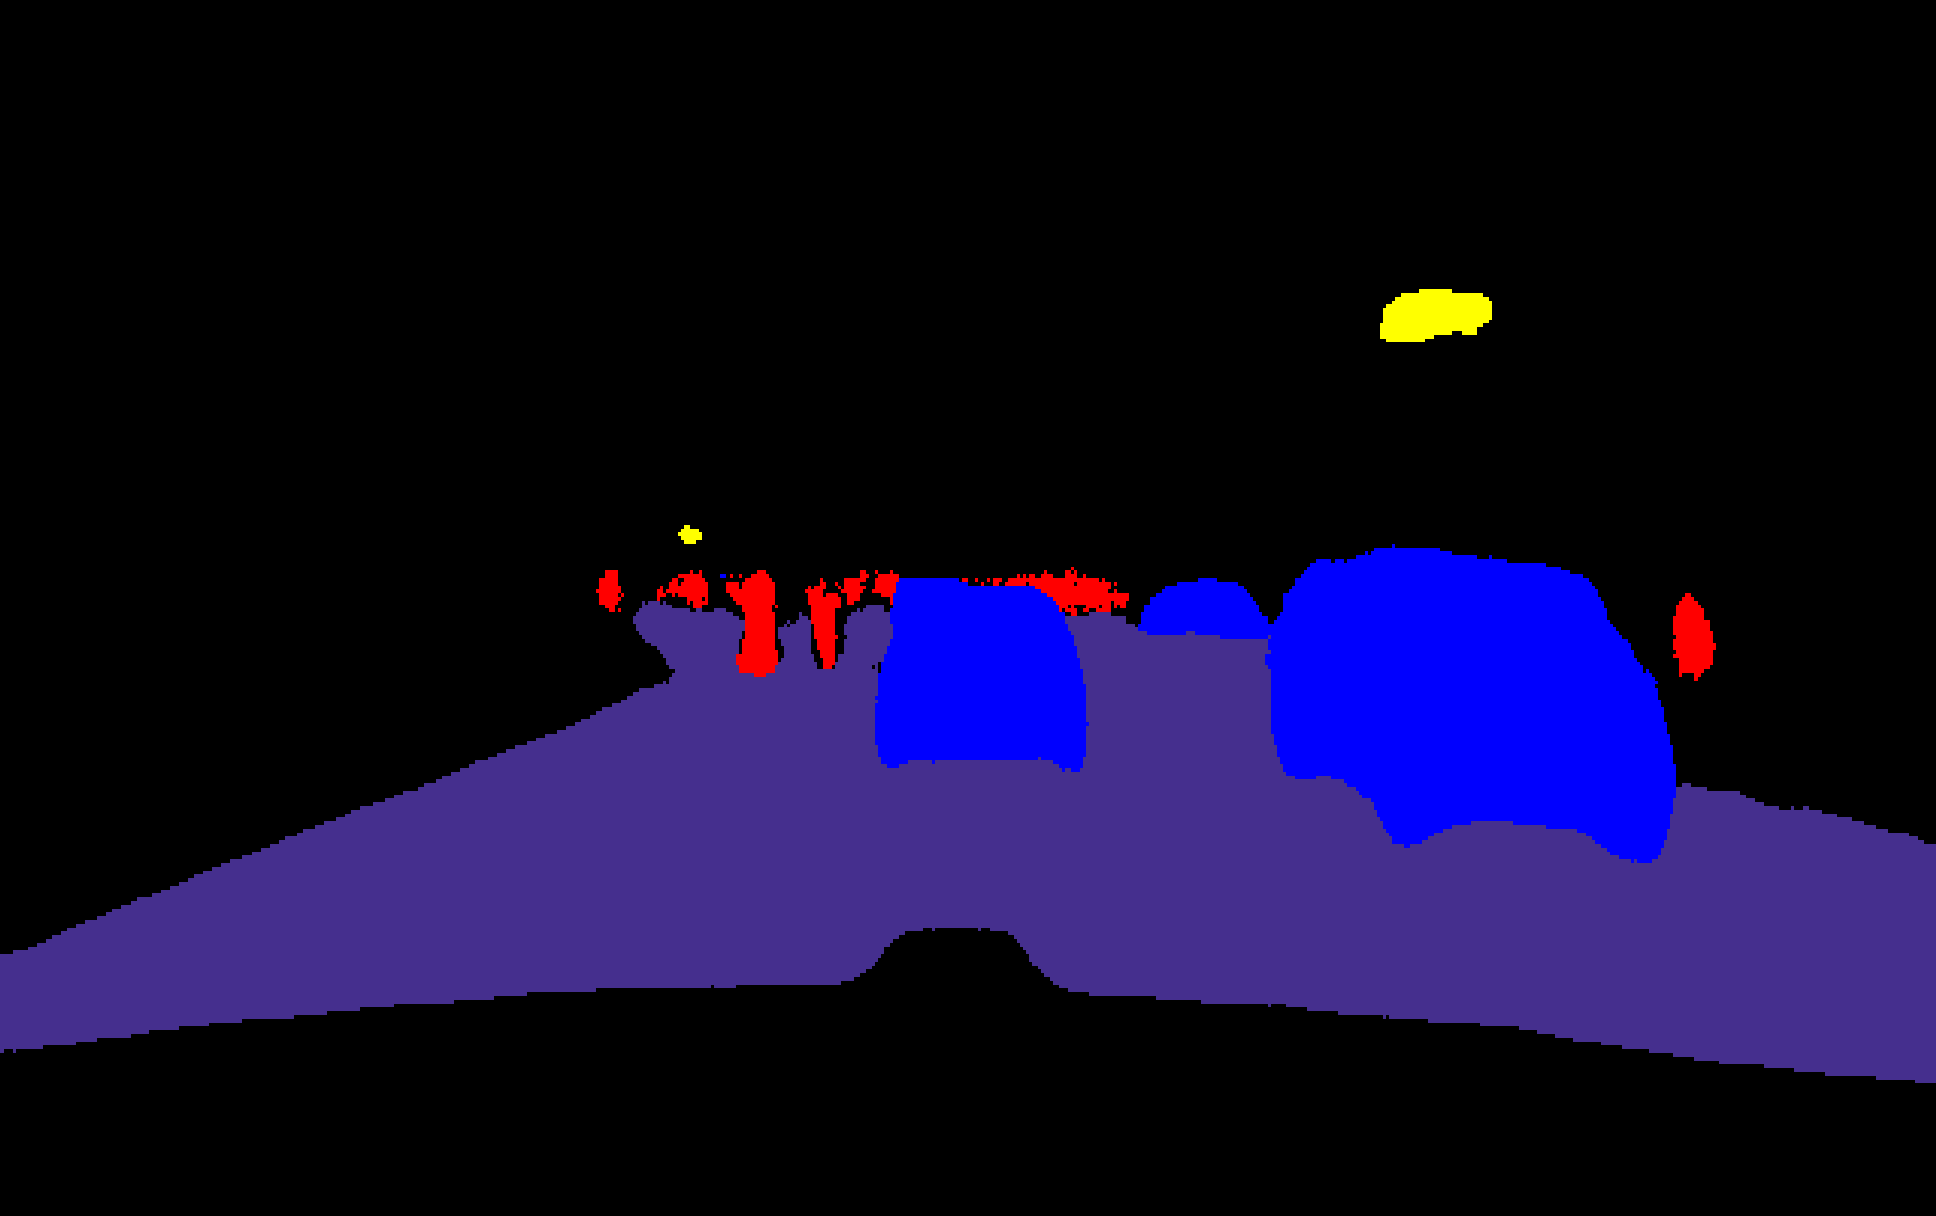
\includegraphics[width=60mm]{./figures/label.png}
     \end{center}
    \end{minipage}
    \begin{minipage}{0.33\hsize}
        \begin{center}
         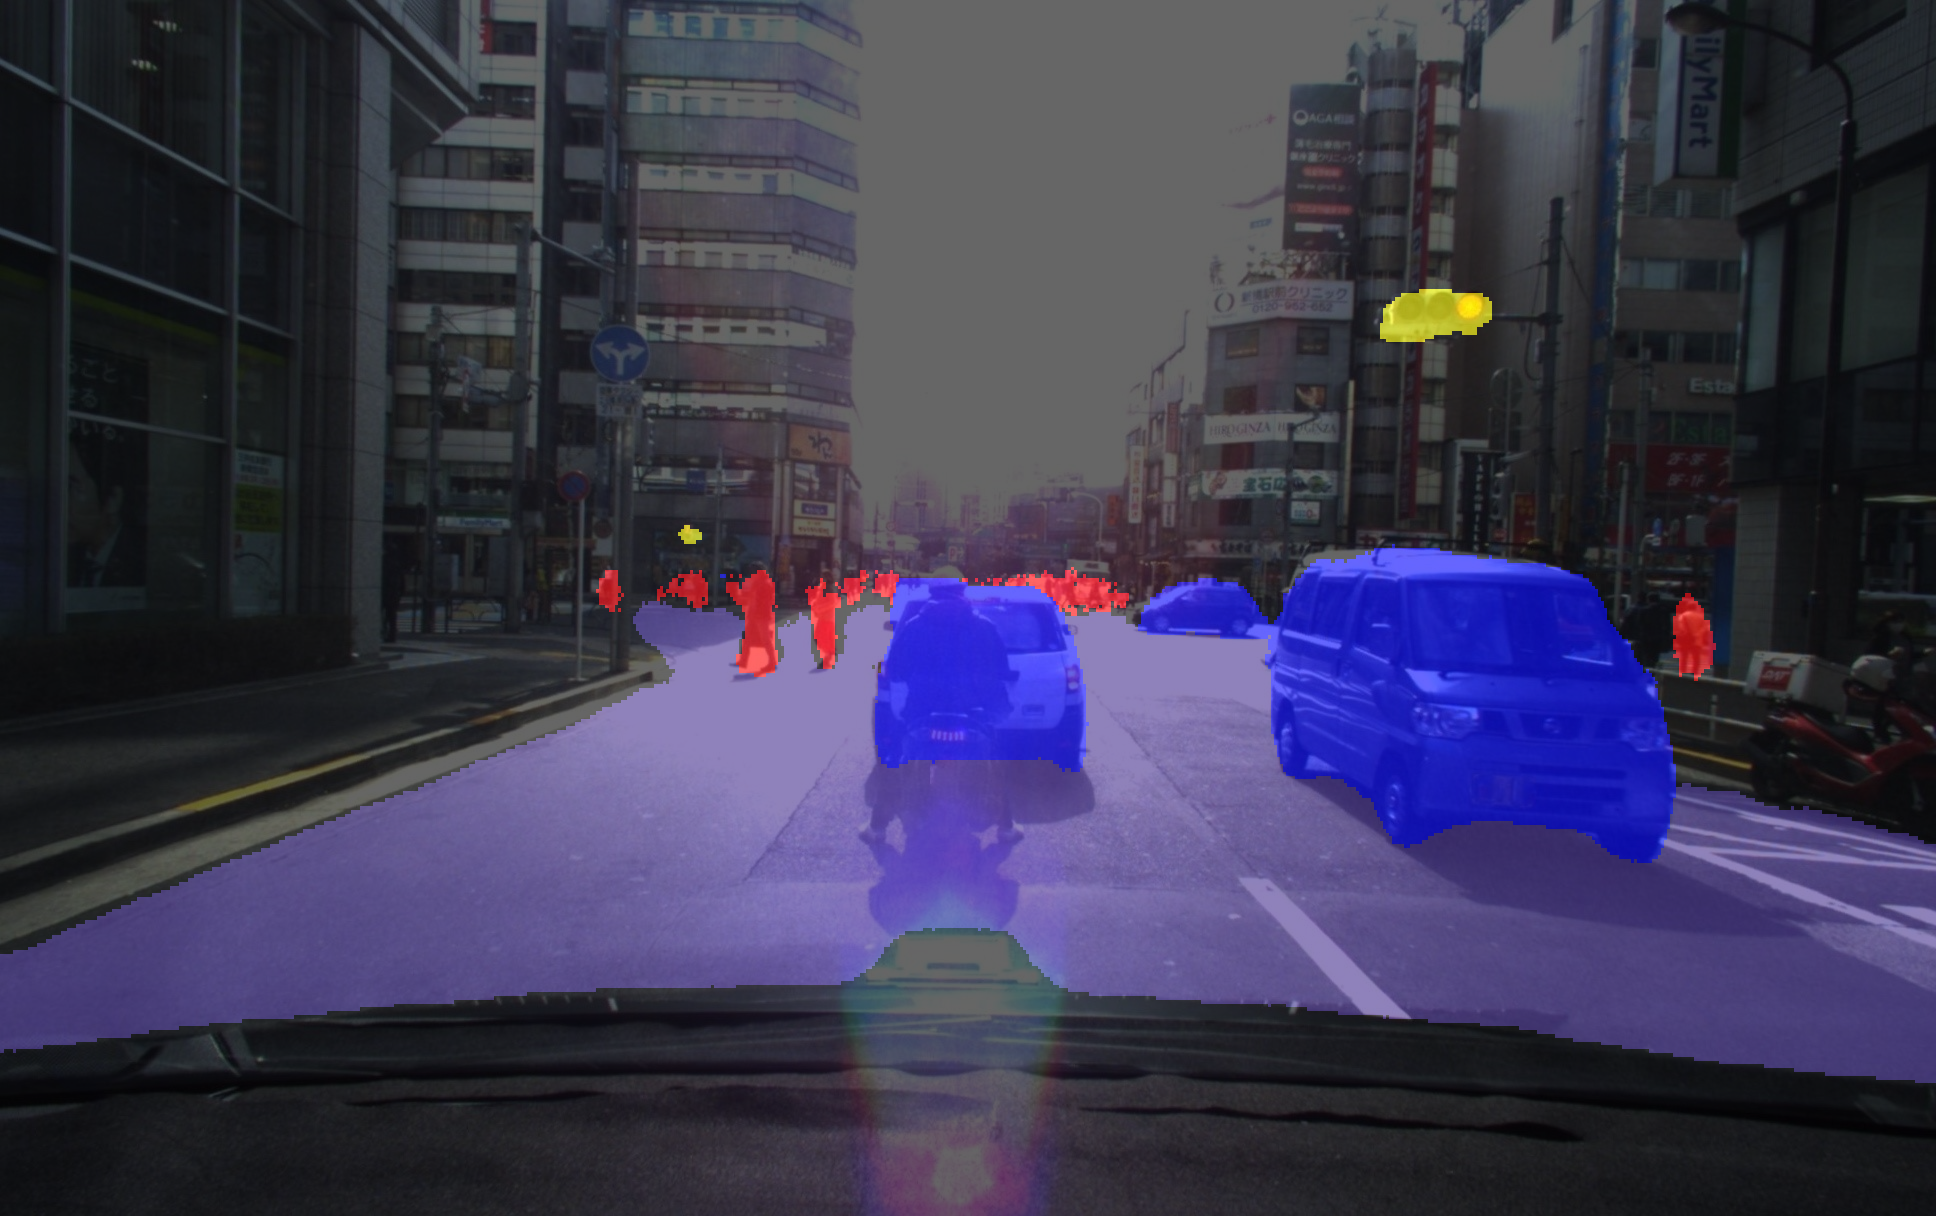
\includegraphics[width=60mm]{./figures/mixed.png}
        \end{center}
       \end{minipage}   
   \end{figure}
推論結果をSIGNATEに投稿した結果,mIoUスコアは0.6014857となった.

\subsection{リソース使用率}
B2304 DPUを第3章で説明したとおりのコンフィグレーションで実装した場合のDPUおよび回路全体のリソース使用率を表\ref{resource_util}に示す.
DPU IPを含んだVivadoプロジェクトをVitisが自動生成する際にベースとするプラットフォームプロジェクトにAXI GPIOやUARTなどのIPが含まれているため,今回のコンテストにおいては不要なIPも含まれている.

\begin{table}[b]
    \begin{center}
        \label{resource_util}
        \caption{リソース使用率}
        \begin{tabular}{lllllllll}
            & Total LUT & Logic LUT & LUTRAM & SRL  & FF    & RAMB36 & RAMB18 & DSP \\ \hline
        DPU & 35175     & 31982     & 1618   & 1575 & 61635 & 147    & 29     & 290 \\ \hline
        ALL & 50414     & 45964     & 2450   & 2000 & 80647 & 151    & 29     & 290
        \end{tabular}
    \end{center}
\end{table}
\subsection{消費電力}
Ultra96V2ボードに供給されるDC電源プラグに流れる電流から,消費電力を計測した.
計測値はアイドル時9.49W,推論時平均11.52W,推論時ピーク12.27Wとなった.